\documentclass[11pt]{article}

\usepackage{fullpage}
\usepackage{rotating}   
\usepackage{amsmath}
\usepackage{amssymb}
\usepackage{amsthm}
\usepackage{fancyhdr}
\usepackage{algorithm}
\usepackage{algorithmic}
\usepackage{bm}
\usepackage{listings}
\usepackage{graphicx}
\usepackage{caption2}
\usepackage{subfigure}
\usepackage{float}
\usepackage{extpfeil}
\usepackage{color}
\usepackage[usenames,dvipsnames]{xcolor}


\newtheorem{theorem}{Theorem}[section]
\newtheorem{lemma}[theorem]{Lemma}
\newtheorem{corollary}[theorem]{Corollary}
\newtheorem{proposition}[theorem]{Proposition}
\newtheorem{definition}[theorem]{Definition}
\newtheorem{conjecture}[theorem]{Conjecture}
\newtheorem{remark}[subsection]{Remark}

%%
\newcommand\numberthis{\addtocounter{equation}{1}\tag{\theequation}}

%% define new symbols
\def\bx{\bm{x}}
\def\bb{\bm{b}}
\def\ba{\bm{a}}
\def\bc{\bm{c}}
\def\bf{\bm{f}}
\def\by{\bm{y}}
\def\bu{\bm{u}}
\def\bv{\bm{v}}
\def\BW{\bm{W}}
\def\BA{\bm{A}}
\def\bz{\bm{z}}
\def\BZ{\bm{Z}}
\def\BH{\bm{H}}
\def\BL{\bm{L}}
\def\BU{\bm{U}}
\def\BV{\bm{V}}
\def\BB{\bm{B}}
\def\BC{\bm{C}}
\def\BD{\bm{D}}
\def\BE{\bm{E}}
\def\BW{\bm{W}}
\def\BQ{\bm{Q}}
\def\BG{\bm{G}}
\def\BA{\bm{A}}
\def\BX{\bm{X}}
\def\BY{\bm{Y}}
\def\BQ{\bm{Q}}
\def\BI{\bm{I}}
\def\BR{\bm{R}}

%% define new brackets
\def\la{\left\langle}
\def\ra{\right\rangle}
\def\ln{\left\|}
\def\rn{\right\|}
\def\lb{\left(}
\def\rb{\right)}
\def\lsb{\left[}
\def\rsb{\right]}
\def\lcb{\left\{}
\def\rcb{\right\}}

%%
\DeclareMathOperator*{\argmin}{arg\,min}
\DeclareMathOperator*{\argmax}{arg\,max}

%%
\title{Homework VIII}
\author{Name: Shao Yanjun, Number: 19307110036}


\begin{document}
\maketitle

%------------------------------------
\begin{abstract}
This is Daniel's homework of  "Numerical Algorithms with Case Studies II".
\end{abstract}
%-------------------------------------
%=====================
\section{Problems}
\paragraph{Q1}
Use the Taylor Theorem, we expand $f(t)$, $f(t+h)$ and $f(t+2h)$ into quadratic term, in a sense that we can not eliminate the cubic term using the linear combination of merely three terms. (We have $a_0=f(t)$, $a_1=f'(t)$ and $a_2=f''(t)$).
\begin{align}
	&f(t)\approx a_0\\
	&f(t+h)\approx a_0+a_1h+a_2h^2\\
	&f(t+2h)\approx a_0+2a_1h+4a_2h^2
\end{align}
Combine (1) and (2), (1) and (3), we will have,
\begin{align}
	&\frac{f(t+2h)-f(t)}{2h}\approx a_1+2a_2h\\
	&\frac{f(t+h)-f(t)}{h}\approx a_1+a_2h
\end{align}
And combine (4) and (5), we will have,
\begin{align}
	2\frac{f(t+h)-f(t)}{h}-\frac{f(t+2h)-f(t)}{2h}=a_1+O(h^2)+O(\frac{u}{h})
\end{align}
Here, $O(h^2)$ is truncation error and $O(\dfrac{u}{h})$ is rounding error. We could adjust the $h$ to minimize the total error.
\paragraph{Q2}
Use Taylor Theorem for multivariables, and expand it to quartic term,
\begin{align}
	g(i,j)&=f(x+i,y+j)-f(x,y)\\
	&\approx h(i\frac{\partial f}{\partial x}+j\frac{\partial f}{\partial y})+\frac{h^2}{2!}(i^2\frac{\partial^2f}{\partial x^2}+2ij\frac{\partial^2f}{\partial xy}+j^2\frac{\partial^2f}{\partial y^2})\\
	&+\frac{h^3}{3!}(i^3\frac{\partial^3f}{\partial x^3}+3i^2j\frac{\partial^3f}{\partial x^2y}+3ij^2\frac{\partial^3f}{\partial xy^2}+j^3\frac{\partial^3f}{\partial y^3})\\
	&+\frac{h^4}{4!}(i^4\frac{\partial^4f}{\partial x^4}+4i^3j\frac{\partial^4f}{\partial x^3y}+6i^2j^2\frac{\partial^4f}{\partial x^2y^2}+4ij^3\frac{\partial^4f}{\partial xy^3}+j^4\frac{\partial^4f}{\partial y^4})
\end{align}
So, we have the following estimation with linear combination,
\begin{align}
fl(\frac{\partial^2f}{\partial x^2}+\frac{\partial^2f}{\partial y^2})&\approx \dfrac{1}{2h^2}(g(1,1)+g(1,-1)+g(-1,1)+g(-1,-1))-2g(0,0)\\
&\approx\frac{\partial^2f}{\partial x^2}+\frac{\partial^2f}{\partial y^2}+O(h^2)
\end{align}
Here, $O(h^2)$ is truncation error.
\paragraph{Q3}
All of the values we obtained through iteration are fairly close to their true values, but we can observe that the result of first iteration is so close that we don't need and can't apply more iterations to get better result. 
\begin{figure}[H]
	\centering
	\subfigure[Richardson extrapolation]{
		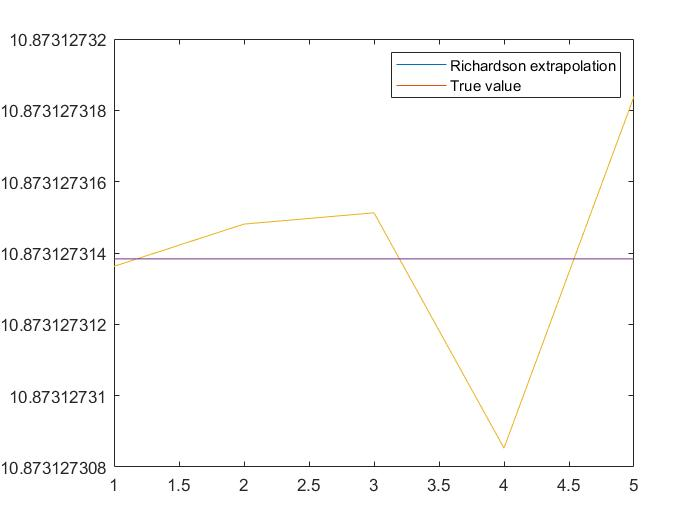
\includegraphics[width=0.4\linewidth]{Richardson.jpg}
	}
\end{figure}
\paragraph{Q4}
As we can see, cubic spline can't have quartic terms or above, so $f'(x)$ can be estimated by 2 iterations of Richardson extrapolation and $f''(x)$ can be calculated by the following method,
\begin{align}
	f''(x)=\frac{f(t+h)+f(t-h)-2f(t)}{h^2}
\end{align}
The spline looks like,
\begin{figure}[H]
	\centering
	\subfigure[spline]{
		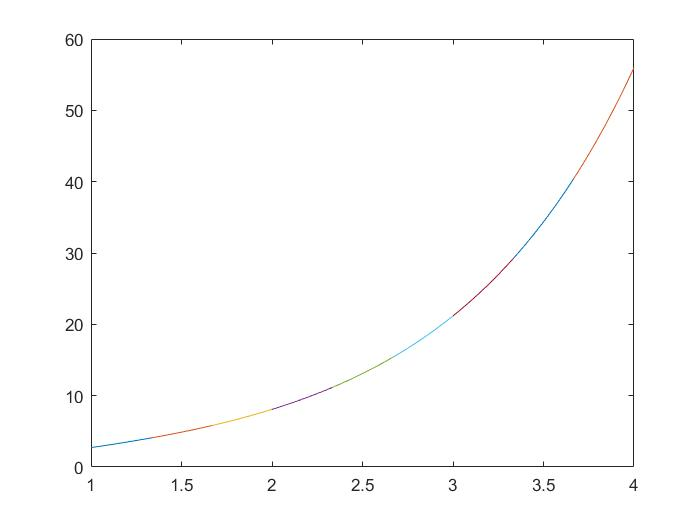
\includegraphics[width=0.4\linewidth]{spline1.jpg}
	}
\end{figure}
We choose stepsize of $h$ as $\{10^{-3},10^{-6},10^{-8},10^{-10}\}$, and the first derivative looks like,
\begin{figure}[H]
	\centering
	\subfigure[first derivative]{
		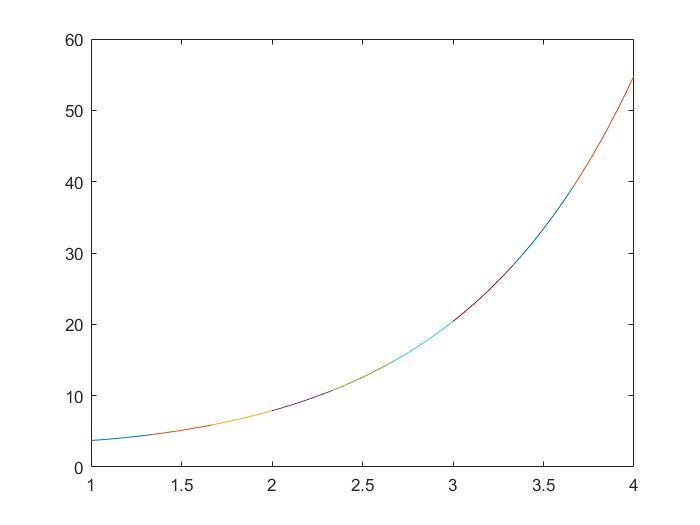
\includegraphics[width=0.4\linewidth]{first derivatives.jpg}
	}
	\subfigure[first derivative error]{
		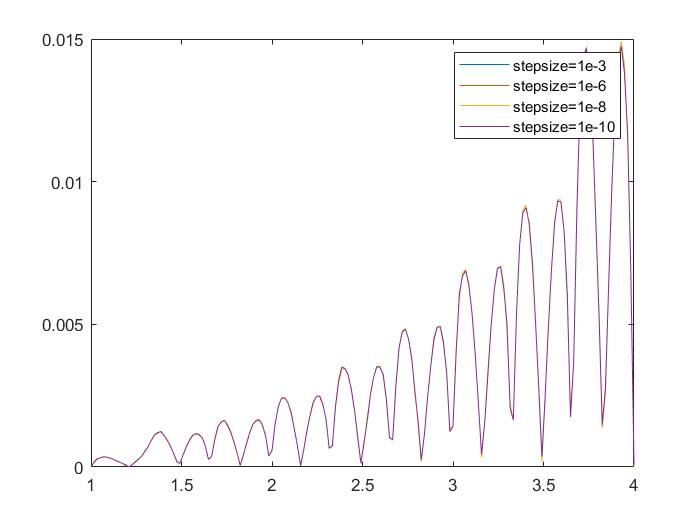
\includegraphics[width=0.4\linewidth]{first derivatives error.jpg}
	}
\end{figure}
But we meet difficulties when trying to find the second derivative with stepsize such as $10^{-8}$ or $10^{-10}\}$.
\begin{figure}[H]
	\centering
	\subfigure[second derivative]{
		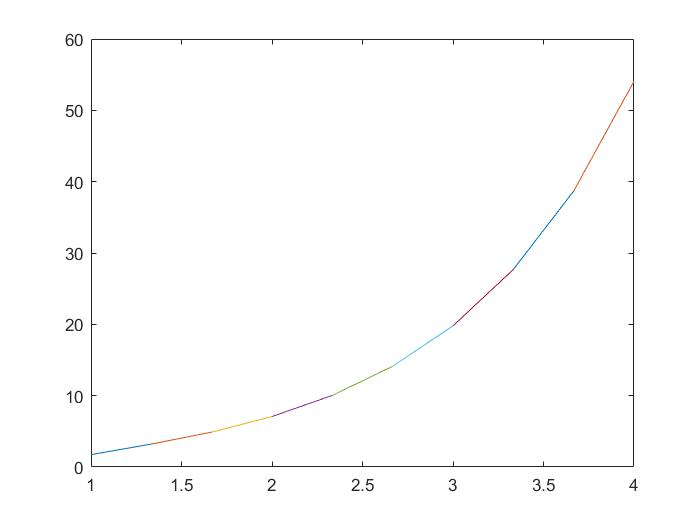
\includegraphics[width=0.4\linewidth]{second derivatives.jpg}
	}
	\subfigure[bad result]{
		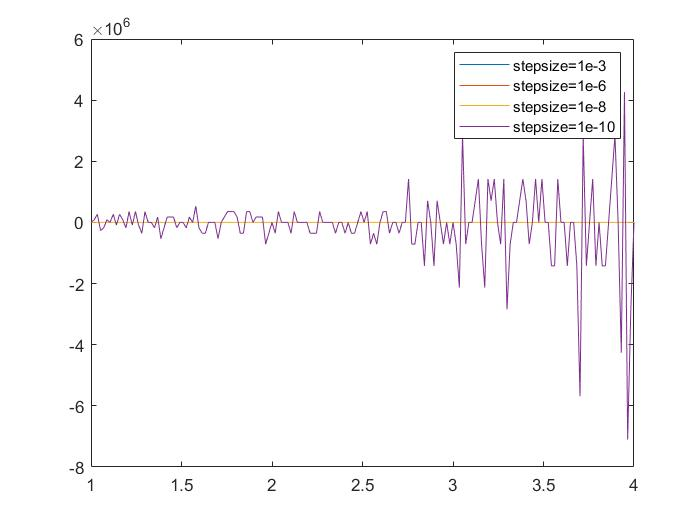
\includegraphics[width=0.4\linewidth]{second derivatives bad.jpg}
	}
\end{figure}
And we remove $10^{-8}$ or $10^{-10}$, the result become beautiful.
\begin{figure}[H]
	\centering
	\subfigure[second derivative error]{
		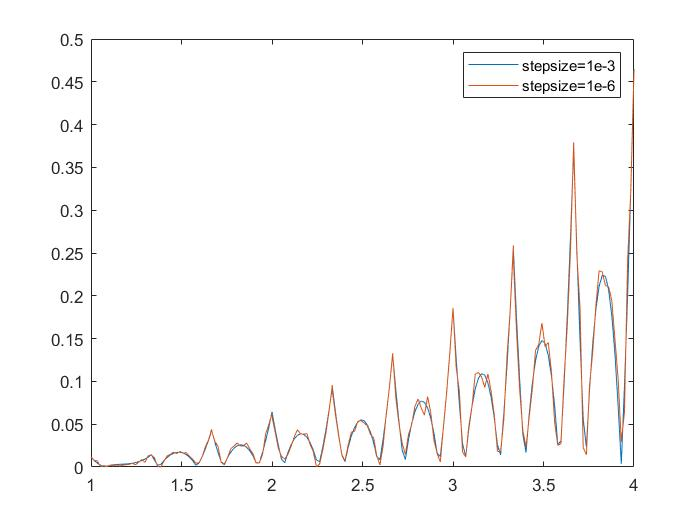
\includegraphics[width=0.4\linewidth]{second derivatives error.jpg}
	}
\end{figure}
That is to say, higher order derivatives are more numerically sensitive to stepsize.
\paragraph{Q5}
The Bezier fitting and cubic spline interpolation should look like the below,
\begin{figure}[H]
	\centering
	\subfigure[Cubic vs Bezier]{
	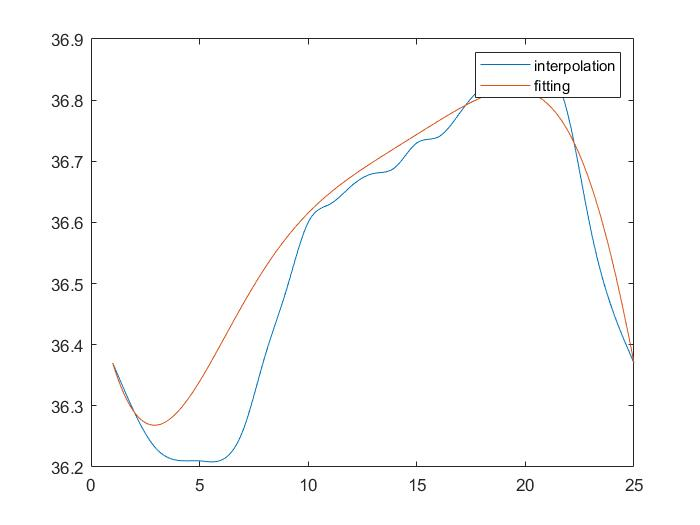
\includegraphics[width=0.4\linewidth]{Bezier vs Cubic.jpg}
}
\end{figure}
The Bezier spline looks more smooth at the first sight.
Plot out our comparison figures for first and second derivatives of fitting and interpolation.
\begin{figure}[H]
	\centering
	\subfigure[first derivative]{
		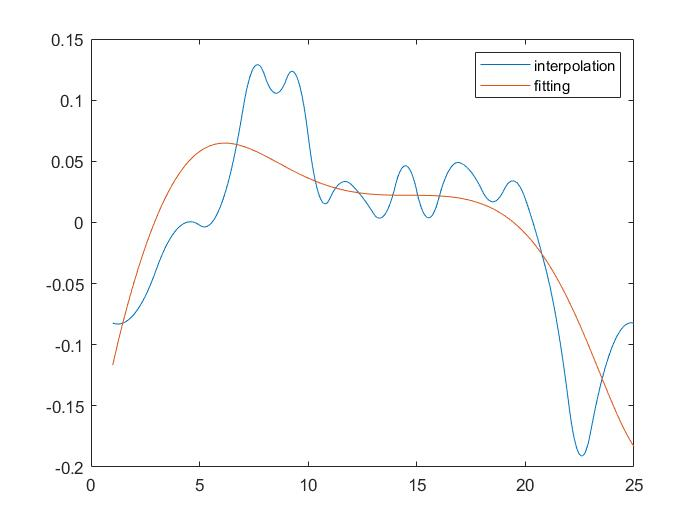
\includegraphics[width=0.4\linewidth]{first derivative.jpg}
	}
	\subfigure[second derivative]{
		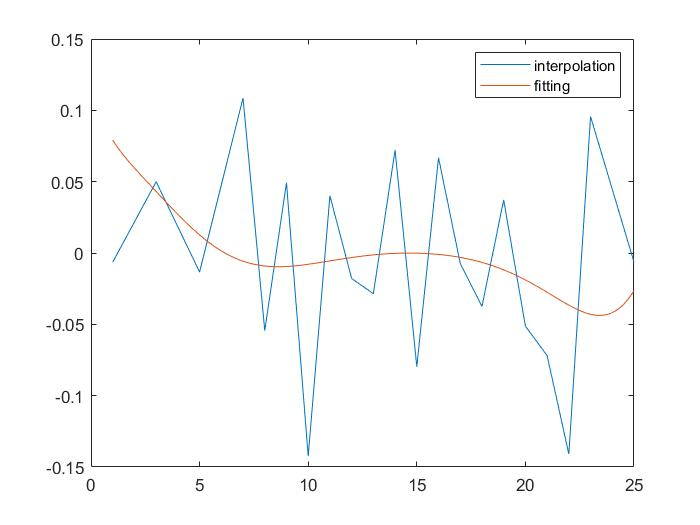
\includegraphics[width=0.4\linewidth]{second derivative.jpg}
	}
\end{figure}
I made choice of the stepsize $h=10^{-3}$ because the second derivative is too sensitive.
\paragraph{Q6}
We construct 8 iterations of Richardson extrapolation, and $n=3*2^{15}$. The convergence is very quick.
\begin{figure}[H]
	\centering
	\subfigure[Converge to $\pi$]{
		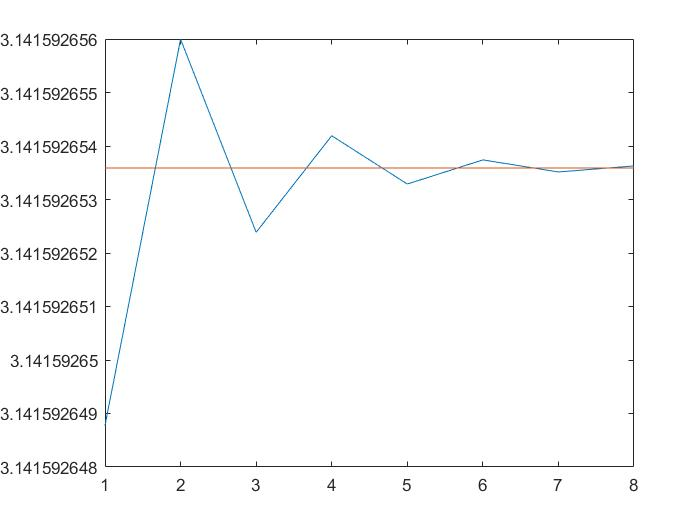
\includegraphics[width=0.4\linewidth]{convergence.jpg}
	}
\end{figure}
%-------------------------------------
%=====================
\end{document}
